\documentclass{jsarticle}
\usepackage{amsmath}
\usepackage{comment}
\usepackage{float}
\usepackage[dvipdfmx,hiresbb]{graphicx}
\usepackage{listings}
\usepackage{float}

\title{ソフトウェア1 lecture6 課題3}
\author{340481H 電子情報工学科内定 中里徳彦}
\date{2014/11/13}
\begin{document}
\maketitle

\section{問題}
\begin{lstlisting}[basicstyle=\ttfamily\footnotesize, frame=single]
#include <stdio.h>

int main()
{
    int **p;
    int *s;
    int a[3][2];
    int i, j;

    p = &s;
    s = &a[0][0];

    for (i = 0; i < 3; i++) {
        for (j = 0; j < 2; j++) {
            a[i][j] = 2*i + j;
        }
    }
    
    printf("%d %d %d %d\n", **p, **(p+1), *(s+1), *(*(a+2)+1));
    return 0;
}
\end{lstlisting}

上のプログラムをみて次の問題に答えよ。

\begin{enumerate}
	\item 5行目のint **p; と 19行目の **pの意味の違いについて述べよ。
	\item p,s,aの関係を図で表せ。
	\item 19行目の出力結果を書け。
	\item a[3][2]がどのような構造になっているか、プログラム終了時にどのような数が入っているかを図で書け。
	\item 19行目をaを用いてポインタを使わずわかりやすく書き直せ。ただし出力結果が不定となる場合はのぞいてよい。
\end{enumerate}

\section{回答}
\begin{enumerate}
	\item int **p;はint型変数のアドレスを持つポインタのアドレスを持つポインタをメモリに確保することを表している。**pはアドレスpにあるポインタsが持っているアドレスにあるint型変数の値を返すという意味である。
	\item 下にある図の通り
	\item 0 不定 1 5
	\item \begin{verbatim}[[0][1]] [[2][3]] [[4][5]] \end{verbatim}
	\item \begin{verbatim}printf("%d %d %d\n", a[0][0], a[0][1], a[2][1]);\end{verbatim}
\end{enumerate}
\begin{figure}[H]
	\centering
	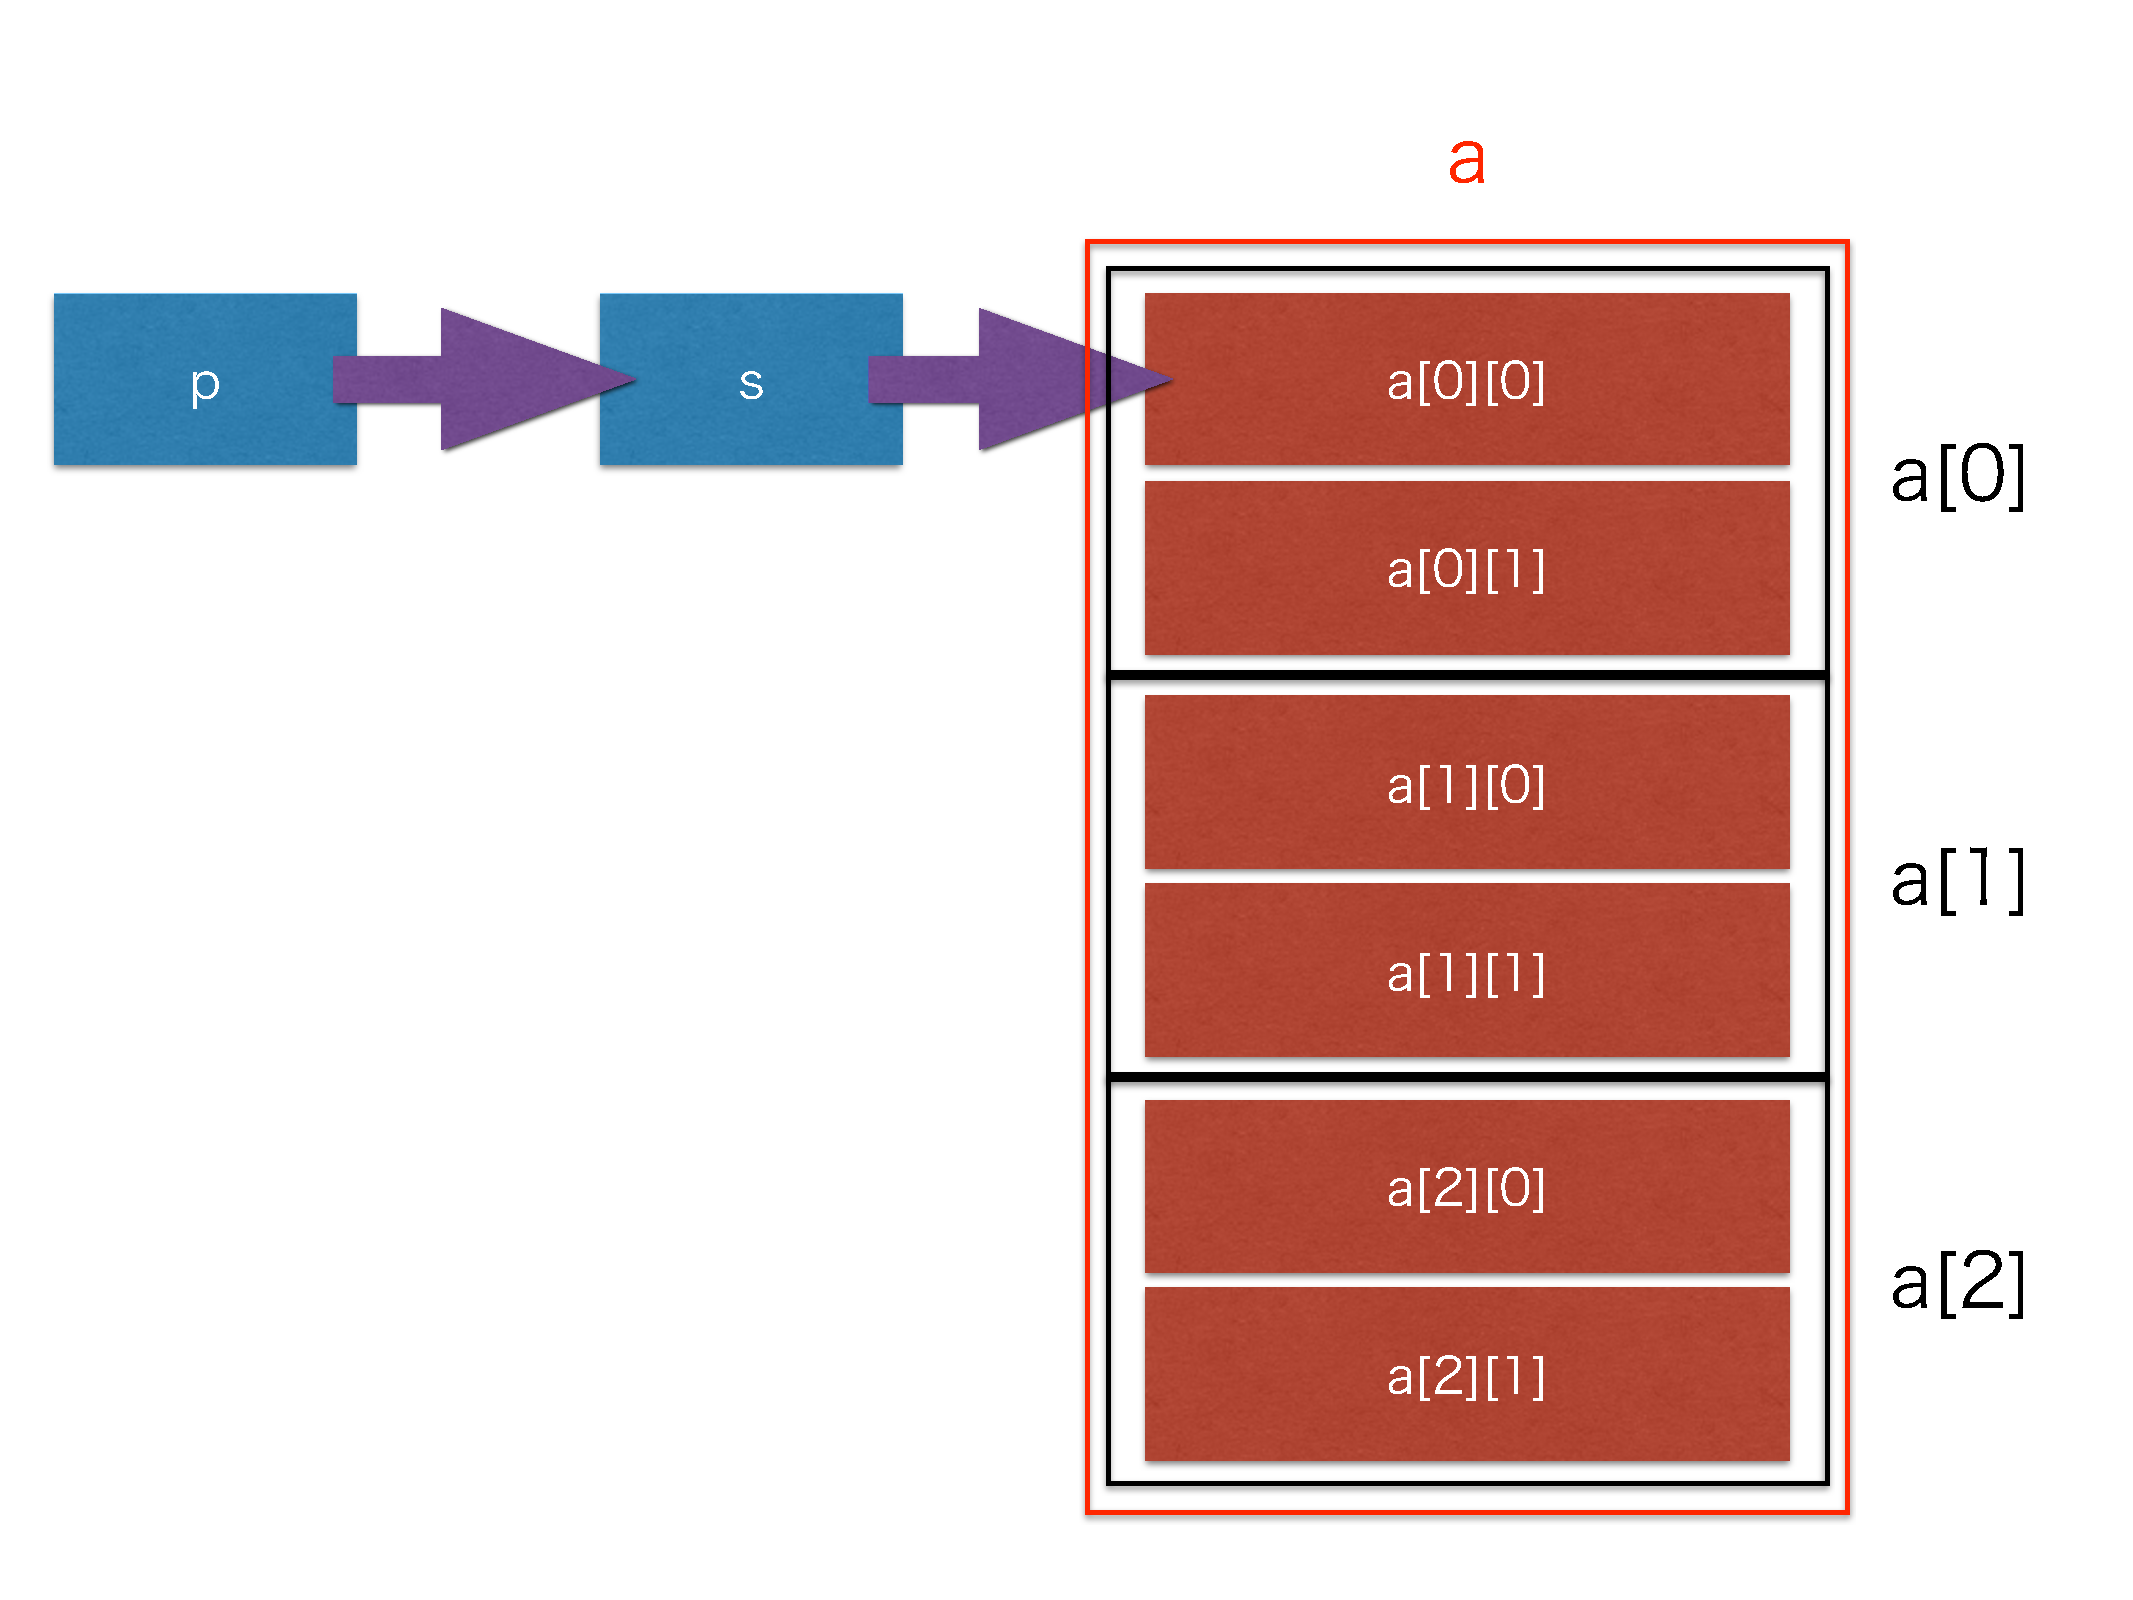
\includegraphics[width=6cm]{assign03_1}
\end{figure}%

\section{効果的と考える理由}
\begin{enumerate}
	\item C言語のポインタがわかりずらい理由の一つは、同じ表現であっても式と宣言で全く違う意味になることがあるからであり、それを問うことでポインタをどの程度理解しているかを把握できると考えた。
	\item どのポインタがどの変数を指すのかがわかるのは、ポインタで最も基本的な部分でありそれを問うことは重要だと思うから。
	\item ポインタ演算がどのような結果を示すかを理解していることは、配列とポインタの関係を理解するうえで重要だから。
	\item a[3][2]が要素数2のint型配列が3つ並んだ配列を意味するのか、それとも、要素数3のint型配列が2つ並んだ配列を意味するのかがわかりにくいから。
	\item ポインタ演算の直感的なわかりにくさを配列を用いて表現した場合と比較することで理解する。
\end{enumerate}
\end{document}